\documentclass[10pt,compress,t,notes=noshow, xcolor=table]{beamer}

% graphicx and color are loaded via lmu-lecture.sty
% maxwidth is the original width if it is less than linewidth
% otherwise use linewidth (to make sure the graphics do not exceed the margin)
% TODO: Remove once cleared to be superfluous
% \makeatletter
% \def\maxwidth{ %
%   \ifdim\Gin@nat@width>\linewidth
%     \linewidth
%   \else
%     \Gin@nat@width
%   \fi
% }
% \makeatother

% ---------------------------------%
% latex-math dependencies, do not remove:
% - mathtools
% - bm
% - siunitx
% - dsfont
% - xspace
% ---------------------------------%

%--------------------------------------------------------%
%       Language, encoding, typography
%--------------------------------------------------------%

\usepackage[english]{babel}
\usepackage[utf8]{inputenc} % Enables inputting UTF-8 symbols
% Standard AMS suite (loaded via lmu-lecture.sty)

% Font for double-stroke / blackboard letters for sets of numbers (N, R, ...)
% Distribution name is "doublestroke"
% According to https://mirror.physik.tu-berlin.de/pub/CTAN/fonts/doublestroke/dsdoc.pdf
% the "bbm" package does a similar thing and may be superfluous.
% Required for latex-math
\usepackage{dsfont}

% bbm – "Blackboard-style" cm fonts (https://www.ctan.org/pkg/bbm)
% Used to be in common.tex, loaded directly after this file
% Maybe superfluous given dsfont is loaded
% TODO: Check if really unused?
% \usepackage{bbm}

% bm – Access bold symbols in maths mode - https://ctan.org/pkg/bm
% Required for latex-math, preferred over \boldsymbol
% https://tex.stackexchange.com/questions/3238/bm-package-versus-boldsymbol
\usepackage{bm}

% pifont – Access to PostScript standard Symbol and Dingbats fonts
% Used for \newcommand{\xmark}{\ding{55}, which is never used
% aside from lecture_advml/attic/xx-automl/slides.Rnw
% \usepackage{pifont}

% Quotes (inline and display), provdes \enquote
% https://ctan.org/pkg/csquotes
\usepackage{csquotes}

% Adds arg to enumerate env, technically superseded by enumitem according
% to https://ctan.org/pkg/enumerate
% Replace with https://ctan.org/pkg/enumitem ?
% Even better: enumitem is not really compatible with beamer and breaks all sorts of things
% particularly the enumerate environment. The enumerate package also just isn't required
% from what I can tell so... don't re-add it I guess?
% \usepackage{enumerate}

% Line spacing - provides \singlespacing \doublespacing \onehalfspacing
% https://ctan.org/pkg/setspace
% \usepackage{setspace}

% mathtools – Mathematical tools to use with amsmath
% https://ctan.org/pkg/mathtools?lang=en
% latex-math dependency according to latex-math repo
\usepackage{mathtools}

% Maybe not great to use this https://tex.stackexchange.com/a/197/19093
% Use align instead -- TODO: Global search & replace to check, eqnarray is used a lot
% $ rg -f -u "\begin{eqnarray" -l | grep -v attic | awk -F '/' '{print $1}' | sort | uniq -c
%   13 lecture_advml
%   14 lecture_i2ml
%    2 lecture_iml
%   27 lecture_optimization
%   45 lecture_sl
\usepackage{eqnarray}
% For shaded regions / boxes
% Used sometimes in optim
% https://www.ctan.org/pkg/framed
\usepackage{framed}

%--------------------------------------------------------%
%       Cite button (version 2024-05)
%--------------------------------------------------------%

% Superseded by style/ref-buttons.sty, kept just in case these don't work out somehow.

% Note this requires biber to be in $PATH when running,
% telltale error in log would be e.g. Package biblatex Info: ... file 'authoryear.dbx' not found
% aside from obvious "biber: command not found" or similar.
% Tried moving this to lmu-lecture.sty but had issues I didn't quite understood,
% so it's here for now.

\usepackage{hyperref}

% Only try adding a references file if it exists, otherwise
% this would compile error when references.bib is not found
% NOTE: Bibliography packages (usebib, biblatex) are now loaded by ref-buttons.sty when needed
% This keeps all bibliography-related setup in one place

% Legacy \citelink command removed - superseded by ref-buttons.sty

%--------------------------------------------------------%
%       Displaying code and algorithms
%--------------------------------------------------------%

% Reimplements verbatim environments: https://ctan.org/pkg/verbatim
% verbatim used sed at least once in
% supervised-classification/slides-classification-tasks.tex
% Removed since code should not be put on slides anyway
% \usepackage{verbatim}

% Both used together for algorithm typesetting, see also overleaf: https://www.overleaf.com/learn/latex/Algorithms
% algorithmic env is also used, but part of the bundle:
%   "algpseudocode is part of the algorithmicx bundle, it gives you an improved version of algorithmic besides providing some other features"
% According to https://tex.stackexchange.com/questions/229355/algorithm-algorithmic-algorithmicx-algorithm2e-algpseudocode-confused
\usepackage{algorithm}
\usepackage{algpseudocode}

%--------------------------------------------------------%
%       Tables
%--------------------------------------------------------%

% multi-row table cells: https://www.namsu.de/Extra/pakete/Multirow.html
% Provides \multirow
% Used e.g. in evaluation/slides-evaluation-measures-classification.tex
\usepackage{multirow}

% colortbl: https://ctan.org/pkg/colortbl
% "The package allows rows and columns to be coloured, and even individual cells." well.
% Provides \columncolor and \rowcolor
% \rowcolor is used multiple times, e.g. in knn/slides-knn.tex
\usepackage{colortbl}

% long/multi-page tables: https://texdoc.org/serve/longtable.pdf/0
% Not used in slides
% \usepackage{longtable}

% pretty table env: https://ctan.org/pkg/booktabs
% Is used
% Defines \toprule
\usepackage{booktabs}

%--------------------------------------------------------%
%       Figures: Creating, placing, verbing
%--------------------------------------------------------%

% wrapfig - Wrapping text around figures https://de.overleaf.com/learn/latex/Wrapping_text_around_figures
% Provides wrapfigure environment -used in lecture_optimization
\usepackage{wrapfig}

% Sub figures in figures and tables
% https://ctan.org/pkg/subfig -- supersedes subfigure package
% Provides \subfigure
% \subfigure not used in slides but slides-tuning-practical.pdf errors without this pkg, error due to \captionsetup undefined
\usepackage{subfig}

% Actually it's pronounced PGF https://en.wikibooks.org/wiki/LaTeX/PGF/TikZ
\usepackage{tikz}

% No idea what/why these settings are what they are but I assume they're there on purpose
\usetikzlibrary{shapes,arrows,automata,positioning,calc,chains,trees, shadows}
\tikzset{
  %Define standard arrow tip
  >=stealth',
  %Define style for boxes
  punkt/.style={
    rectangle,
    rounded corners,
    draw=black, very thick,
    text width=6.5em,
    minimum height=2em,
    text centered},
  % Define arrow style
  pil/.style={
    ->,
    thick,
    shorten <=2pt,
    shorten >=2pt,}
}

%--------------------------------------------------------%
%       Beamer setup and custom macros & environments
%--------------------------------------------------------%

% Main sty file for beamer setup (layout, style, lecture page numbering, etc.)
% For long-term maintenance, this may me refactored into a more modular set of .sty files
\usepackage{../../style/lmu-lecture}
% Custom itemize wrappers, itemizeS, itemizeL, etc
\usepackage{../../style/customitemize}
% Custom framei environment, uses custom itemize!
\usepackage{../../style/framei}
% Custom frame2 environment, allows specifying font size for all content
\usepackage{../../style/frame2}
% Column layout macros
\usepackage{../../style/splitV}
% \image and derivatives
\usepackage{../../style/image}
% New generation of reference button macros
\usepackage{../../style/ref-buttons}

% Used regularly
\let\code=\texttt

% Not sure what/why this does
\setkeys{Gin}{width=0.9\textwidth}

% -- knitr leftovers --
% These may be used by knitr/R Markdown workflows in other lectures
\makeatletter
\def\maxwidth{ %
  \ifdim\Gin@nat@width>\linewidth
    \linewidth
  \else
    \Gin@nat@width
  \fi
}
\makeatother

% Define colors for syntax highlighting (may be used by knitr)
\definecolor{fgcolor}{rgb}{0.345, 0.345, 0.345}
\definecolor{shadecolor}{rgb}{.97, .97, .97}

% knitr code output environment
\newenvironment{knitrout}{}{}


% Can't find a reason why common.tex is not just part of this file?
% This file is included in slides and exercises

% Rarely used fontstyle for R packages, used only in 
% - forests/slides-forests-benchmark.tex
% - exercises/single-exercises/methods_l_1.Rnw
% - slides/cart/attic/slides_extra_trees.Rnw
\newcommand{\pkg}[1]{{\fontseries{b}\selectfont #1}}

% Spacing helpers, used often (mostly in exercises for \dlz)
\newcommand{\lz}{\vspace{0.5cm}} % vertical space (used often in slides)
\newcommand{\dlz}{\vspace{1cm}}  % double vertical space (used often in exercises, never in slides)
\newcommand{\oneliner}[1] % Oneliner for important statements, used e.g. in iml, algods
{\begin{block}{}\begin{center}\begin{Large}#1\end{Large}\end{center}\end{block}}

% Don't know if this is used or needed, remove?
% textcolor that works in mathmode
% https://tex.stackexchange.com/a/261480
% Used e.g. in forests/slides-forests-bagging.tex
% [...] \textcolor{blue}{\tfrac{1}{M}\sum^M_{m} [...]
% \makeatletter
% \renewcommand*{\@textcolor}[3]{%
%   \protect\leavevmode
%   \begingroup
%     \color#1{#2}#3%
%   \endgroup
% }
% \makeatother


% Defines macros and environments
% This file is included in slides and exercises

% Rarely used fontstyle for R packages, used only in 
% - forests/slides-forests-benchmark.tex
% - exercises/single-exercises/methods_l_1.Rnw
% - slides/cart/attic/slides_extra_trees.Rnw
\newcommand{\pkg}[1]{{\fontseries{b}\selectfont #1}}

% Spacing helpers, used often (mostly in exercises for \dlz)
\newcommand{\lz}{\vspace{0.5cm}} % vertical space (used often in slides)
\newcommand{\dlz}{\vspace{1cm}}  % double vertical space (used often in exercises, never in slides)
\newcommand{\oneliner}[1] % Oneliner for important statements, used e.g. in iml, algods
{\begin{block}{}\begin{center}\begin{Large}#1\end{Large}\end{center}\end{block}}

% Don't know if this is used or needed, remove?
% textcolor that works in mathmode
% https://tex.stackexchange.com/a/261480
% Used e.g. in forests/slides-forests-bagging.tex
% [...] \textcolor{blue}{\tfrac{1}{M}\sum^M_{m} [...]
% \makeatletter
% \renewcommand*{\@textcolor}[3]{%
%   \protect\leavevmode
%   \begingroup
%     \color#1{#2}#3%
%   \endgroup
% }
% \makeatother


\title{Interpretable Machine Learning}
% \author{LMU}
%\institute{\href{https://compstat-lmu.github.io/lecture_iml/}{compstat-lmu.github.io/lecture\_iml}}
\date{}

\begin{document}

\titlemeta{
Individual Conditional Expectation (ICE) Plot
}{
Interpretable Machine Learning
}{
figure/feature-effect
}{

%\item Intro to feature effects
\item ICE curves as local effect method
\item How to sample grid points for ICE curves
%\item Understand how to interpret ICE curves and PD plots

}



\begin{frame}{Motivation}
%ICE curves show how different feature values of an observation affect its model prediction \newline $\Rightarrow$ \textbf{local interpretation method}
%From a local perspective, one might be interested in how changing feature values of an observation affect model prediction

\textbf{Question:} How does varying a single feature of an obs. affect its predicted outcome?

\smallskip

\textbf{Idea:} For a given observation, change the value of the feature of interest, and visualize how prediction changes

\smallskip

\textbf{Example:} On model prediction surface (left), select observation and visualize changes in prediction for different values of $x_2$, while keeping $x_1$ fixed \\ $\Rightarrow$ \textbf{local interpretation}

\bigskip
\centering
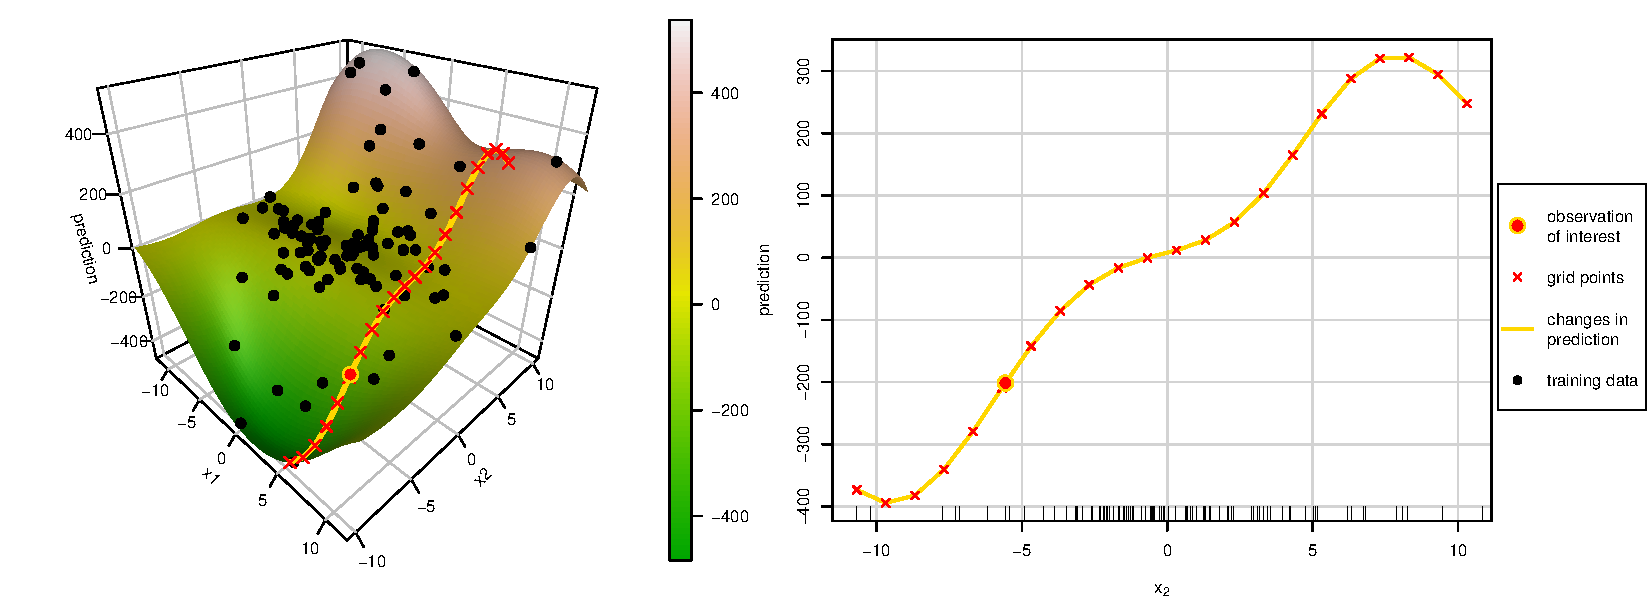
\includegraphics[width=\textwidth]{figure/ice_motivation}

%$\Rightarrow$ Repeat for all observations and average the curves for global feature effect ($\leadsto$ PD plots)
\end{frame}




\begin{frame}[c]{Individual Conditional Expectation (ICE) \furtherreading{Goldstein_2013}}

%Consider an index set $S \subseteq \{1, \dots, p\}$ and its complement $C = S^\complement$.
%\lz
\begin{columns}[T, totalwidth=\textwidth]
\begin{column}{0.16\textwidth} % 0.2 4.26cm
\includegraphics[page=1, trim=0cm 0.35cm 4.53cm 0.35cm, clip, width=0.9\textwidth]{../../figure_man/ice_plot_demo}
\end{column}
\begin{column}{0.84\textwidth}

%%%

%Assume each observation $\xi$ can be partitioned into $\xi_S$ and $\xi_C$ containing only feature values from the index set $S \subseteq \{1, \dots, p\}$ and its complement $C = S^\complement$, respectively.
%Assume each observation $\xi$ can be partitioned into $\xi_S$ and $\xi_C$ containing only feature values addressed by the feature's index set $S \subseteq \{1, \dots, p\}$ and its complement $C = S^\complement$, respectively.
%Assume each observation $\xi$ can be partitioned into $\xi_S$ and $\xi_C$ containing values from features addressed by the index set $S \subseteq \{1, \dots, p\}$ and its complement $C = S^\complement$, respectively.
Partition each observation $\xv$ into $\xv_S$ (feature(s) of interest) and $\xv_{-S}$ (remaining features)
\begin{itemize}
    \item[$\leadsto$] In practice, $\xv_S$ consists of one or two features \\ (i.e., $|S| \leq 2$ and ${-S} = S^\complement$).
    %, containing only feature values indexed by $S \subseteq \{1, \dots, p\}$ and its complement $C = S^\complement$.
\end{itemize}

\medskip

Formal definition of ICE curves: 
\begin{itemize}
    \item Define grid points $\xv_S^* = \xv_S^{*^{(1)}}, \dots, \xv_S^{*^{(g)}}$ to vary $\xv_S$
    \item Plot point pairs $ \Bigl\{\left(\xv_S^{*^{(k)}}, \fhice{S}^{(i)}(\xv_S^{*^{(k)}}) \right) \Bigr\}_{k=1}^g$
    \\where $\fhice{S}^{(i)}(\xv_S^*) = \fh(\xv_S^*, \xi_{-S})$
    \item For each $k$ connect point pairs to obtain \textbf{ICE curve}
\end{itemize}

\medskip

\begin{itemize}
    \item[$\leadsto$] ICE curves visualize how prediction of $i$-th observation changes after varying its feature values indexed by $S$ using grid points $\xv_S^*$ while keeping all values in $-S$ fixed
%by replacing the feature values $\xv_S^{(i)}$ with other values $\xv_S$ while keeping all other features in $\xi_C$ fixed:
%by varying the feature values in $\xv_S$ while keeping all other features in $\xi_C$ fixed.

% \begin{itemize}
%     \item[$\leadsto$] Plot \quad $\fh_{S}^{(i)}(\xv_S^*) \; \text{ vs. } \; \xv_S^*$ \\
%     where $\fh_{S}^{(i)}(\xv_S^*) = \fh(\xv_S^*, \xi_{-S})$ is prediction of $i$-th observation in which original feature value $\xi_S$ was replaced by $\xv_S^*$.
% \end{itemize}
\end{itemize}


%Visualize for \textbf{I}ndividual observations and \textbf{C}onditional on all other features how \textbf{E}xpected prediction changes

\end{column}
\end{columns}

% \begin{columns}[T, totalwidth=\textwidth]
% \begin{column}{0.6\textwidth}


% \end{column}
% \begin{column}{0.4\textwidth}
% %\begin{center}
% \centerline{\includegraphics[width=\textwidth]{figure_man/ice_bike10obs}}
% %\end{center}
% %\vspace{-0.3cm}
% \scriptsize{\textbf{Figure:} ICE Curves of 10 observations of the bike sharing dataset. Each line displays the change in prediction for a single observation due to varying the feature temperature.\par}
%
% \end{column}
% \end{columns}
%\footnote[frame]{Goldstein, A., Kapelner, A., Bleich, J., and Pitkin, E. (2013). Peeking Inside the Black Box: Visualizing Statistical Learning with Plots of Individual Conditional Expectation, 1-22. https://doi.org/10.1080/10618600.2014.907095}
\end{frame}

% \begin{frame}{Individual Conditional Expectation (ICE)}
%
% Steps to create an ICE curve of an observation regarding a single feature $\xv_S$ according to the \textbf{SIPA} framework:
%
% \begin{enumerate}
% \item \textbf{Sampling:} Choose grid points along $\xv_S$.
% \item For each grid point:
% \begin{itemize}
% \item \textbf{Intervention:} Replace the original feature value $\xv_S$ with the current grid value.
% \item \textbf{Prediction:} Get the model prediction with replaced feature value $\xv_S$.
% \end{itemize}
% \item \textbf{Aggregation:} none.
% \item \textbf{Visualization:} Draw a curve per observation with the grid points on the x-axis and the prediction on the y-axis.
% \end{enumerate}
%
% \footnote[frame]{Scholbeck, C. A., Molnar, C., Heumann, C., Bischl, B., and Casalicchio, G. (2019). Sampling, Intervention, Prediction, Aggregation: A Generalized Framework for Model Agnostic Interpretations. ECML PKDD 2019. (pp. 205-216).}
% \end{frame}

% \begin{frame}{Individual Conditional Expectation (ICE)}
%
% \begin{columns}[T, totalwidth=\textwidth]
% \begin{column}{0.4\textwidth}
% \includegraphics[page=1, trim=0cm 0.35cm 0.85cm 0.35cm, width=0.9\textwidth]{figure_man/ice_plot_demo}
% \end{column}
% \begin{column}{0.55\textwidth}
%
% \end{column}
% \end{columns}
% %\vspace*{\topsep}
%
% aa
% \end{frame}

\begin{frame}{ICE Curves - Illustration}

\begin{columns}[c, totalwidth=\textwidth]
\begin{column}{0.4\textwidth}
\includegraphics[page=2, trim=0cm 0.35cm 0.85cm 0.35cm, width=0.9\textwidth]{../../figure_man/ice_plot_demo}
\end{column}
\begin{column}{0.55\textwidth}

\end{column}
\end{columns}
\vspace*{\topsep}

\textbf{1. Step - Grid points:}

%For the $i$-th observation, we
\begin{itemize}
    \item Sample grid values $\xv_S^{*^{(1)}}, \dots, \xv_S^{*^{(g)}}$ along possible values of feature $S$ ($|S| = 1$)
\item For $\xv^{(i)} = (\xv_S, \xv_{-S})$, replace  $\xv_S$ with those grid values
\end{itemize}
%h observation with these sampled grid values.
%$\Rightarrow$ New artificial data points for $i$-th obs.
$\Rightarrow$ Creates new artificial points for $i$-th observation (here: $\xv_S^* = x_1^* \in \{1, 2, 3\}$ scalar)

\end{frame}

\begin{frame}{ICE Curves - Illustration}

\begin{columns}[c, totalwidth=\textwidth]
\begin{column}{0.4\textwidth}
\includegraphics<1>[page=3, trim=0cm 0.35cm 0.85cm 0.35cm, width=0.9\textwidth]{../../figure_man/ice_plot_demo}
\includegraphics<2>[page=4, trim=0cm 0.35cm 0.85cm 0.35cm, width=0.9\textwidth]{../../figure_man/ice_plot_demo}
\includegraphics<3>[page=5, trim=0cm 0.35cm 0.85cm 0.35cm, width=0.9\textwidth]{../../figure_man/ice_plot_demo}
\end{column}
\begin{column}{0.55\textwidth}
\includegraphics<1>[page=1, width=0.85\textwidth]{figure/ICE}
\includegraphics<2>[page=2, width=0.85\textwidth]{figure/ICE}
\includegraphics<3>[page=3, width=0.85\textwidth]{figure/ICE}
\end{column}
\end{columns}
\vspace*{\topsep}

\textbf{2. Step - Predict and visualize:}

For each artificially created data point of $i$-th observation, plot prediction $\fhice{S}^{(i)}(\xv_S^*)$ vs. grid values $\xv_S^*$:

$$\fhice{1}^{(i)}(x_1^*) = \fh(x_1^*, \xi_{2, 3}) \text{ vs. } x_1^* \in \{1, 2, 3\}$$

\end{frame}

% \begin{frame}{Individual Conditional Expectation (ICE)}

% \begin{columns}[T, totalwidth=\textwidth]
% \begin{column}{0.4\textwidth}
% \includegraphics[page=4, trim=0cm 0.35cm 0.85cm 0.35cm, width=0.9\textwidth]{figure_man/ice_plot_demo}
% \end{column}
% \begin{column}{0.55\textwidth}
% \includegraphics[page=2, width=0.85\textwidth]{figure/ICE}
% \end{column}
% \end{columns}
% \vspace*{\topsep}

% \textbf{Predict and visualize:}

% For each artificially created data point of $i$-th observation, plot prediction $\fh_{S}^{(i)}(\xv_S^*)$ vs. grid values $\xv_S^*$:

% $$\fh_{1}^{(i)}(x_1^*) = \fh(x_1^*, \xi_{2, 3}) \text{ vs. } x_1^* \in \{1, 2, 3\}$$
% \end{frame}

% \begin{frame}{Individual Conditional Expectation (ICE)}

% \begin{columns}[T, totalwidth=\textwidth]
% \begin{column}{0.4\textwidth}
% \includegraphics[page=5, trim=0cm 0.35cm 0.85cm 0.35cm, width=0.9\textwidth]{figure_man/ice_plot_demo}
% \end{column}
% \begin{column}{0.55\textwidth}
% \includegraphics[page=3, width=0.85\textwidth]{figure/ICE}
% \end{column}
% \end{columns}
% \vspace*{\topsep}

% \textbf{Predict and visualize:}

% For each artificially created data point of $i$-th observation, plot prediction $\fh_{S}^{(i)}(\xv_S^*)$ vs. grid values $\xv_S^*$:

% $$\fh_{1}^{(i)}(x_1^*) = \fh(x_1^*, \xi_{2, 3}) \text{ vs. } x_1^* \in \{1, 2, 3\}$$
% \end{frame}

% \begin{frame}{Individual Conditional Expectation (ICE)}

% % \begin{columns}[T]
% % \begin{column}{0.4\textwidth}
% % \includegraphics[page=5, trim=0cm 0.35cm 0.85cm 0.35cm, width=0.9\textwidth]{figure_man/ice_plot_demo}
% % \end{column}
% % \begin{column}{0.55\textwidth}
% % \includegraphics[page=3, width=0.85\textwidth]{figure/ICE}
% % \end{column}
% % \end{columns}
% % \vspace*{\topsep}

% \begin{itemize}
%     \item \textbf{Interpretation:} \textbf{ICE} curve visualizes for \textbf{I}ndividual observations and \textbf{C}onditional on all other features (by keeping all other features constant) how \textbf{E}xpected prediction changes
%     \item
%     \item For global view, repeat procedure for all observations
% \end{itemize}

% % \textbf{Definition:}

% % ICE curves involve plotting the pairs $ \{(\xv_S^{*^{(k)}}, \fh_{S}^{(i)}(\xv_S^*{^{(k)}})) \}_{k=1}^g $ for grid points $\xv_S^{*^{(1)}}, \dots, \xv_S^{*^{(g)}}$.
% \end{frame}

\begin{frame}{ICE Curves - Illustration}

\begin{columns}[T, totalwidth=\textwidth]
\begin{column}{0.4\textwidth}
\includegraphics<1>[page=6, trim=0cm 0.35cm 0.85cm 0.35cm, width=0.9\textwidth]{../../figure_man/ice_plot_demo}
\includegraphics<2>[page=7, trim=0cm 0.35cm 0.85cm 0.35cm, width=0.9\textwidth]{../../figure_man/ice_plot_demo}
\end{column}
\begin{column}{0.55\textwidth}
\includegraphics<1>[page=4, width=0.85\textwidth]{figure/ICE}
\includegraphics<2>[page=5, width=0.85\textwidth]{figure/ICE}
\end{column}
\end{columns}
\vspace*{\topsep}

\textbf{3. Step - Repeat for other observations:}

ICE curve for\only<1>{ $i=2$ }\only<2>{ $i=3$ }connects all predictions at grid values associated to $i$-th obs.
\end{frame}

% \begin{frame}{ICE Curves - Illustration}

% \begin{columns}[T, totalwidth=\textwidth]
% \begin{column}{0.4\textwidth}
% \includegraphics[page=7, trim=0cm 0.35cm 0.85cm 0.35cm, width=0.9\textwidth]{figure_man/ice_plot_demo}
% \end{column}
% \begin{column}{0.55\textwidth}
% %\begin{center}
% \includegraphics[page=5, width=0.85\textwidth]{figure/ICE}
% %\end{center}
% \end{column}
% \end{columns}
% \vspace*{\topsep}

% \textbf{3. Step - Repeat for other observations:}

% ICE curve for $i=3$ connects all predictions at grid values associated to $i$-th obs.
% %The ICE curve of observation $i=3$ connects all predictions at the corresponding grid values associated to the $i$-th obs.

% % \textbf{Definition:}

% % ICE curves involve plotting the pairs $ \{(\xv_S^{*^{(k)}}, \fh_{S}^{(i)}(\xv_S^*{^{(k)}})) \}_{k=1}^g $ for grid points $\xv_S^{*^{(1)}}, \dots, \xv_S^{*^{(g)}}$.
% \end{frame}

\begin{frame}{ICE Curves - Interpretation}
\textbf{Example:} Prediction surface of a model (left), select observation and visualize changes in prediction for different values of $x_2$ while keeping $x_1$ fixed \\ $\Rightarrow$ \textbf{local interpretation}

\bigskip
\centering
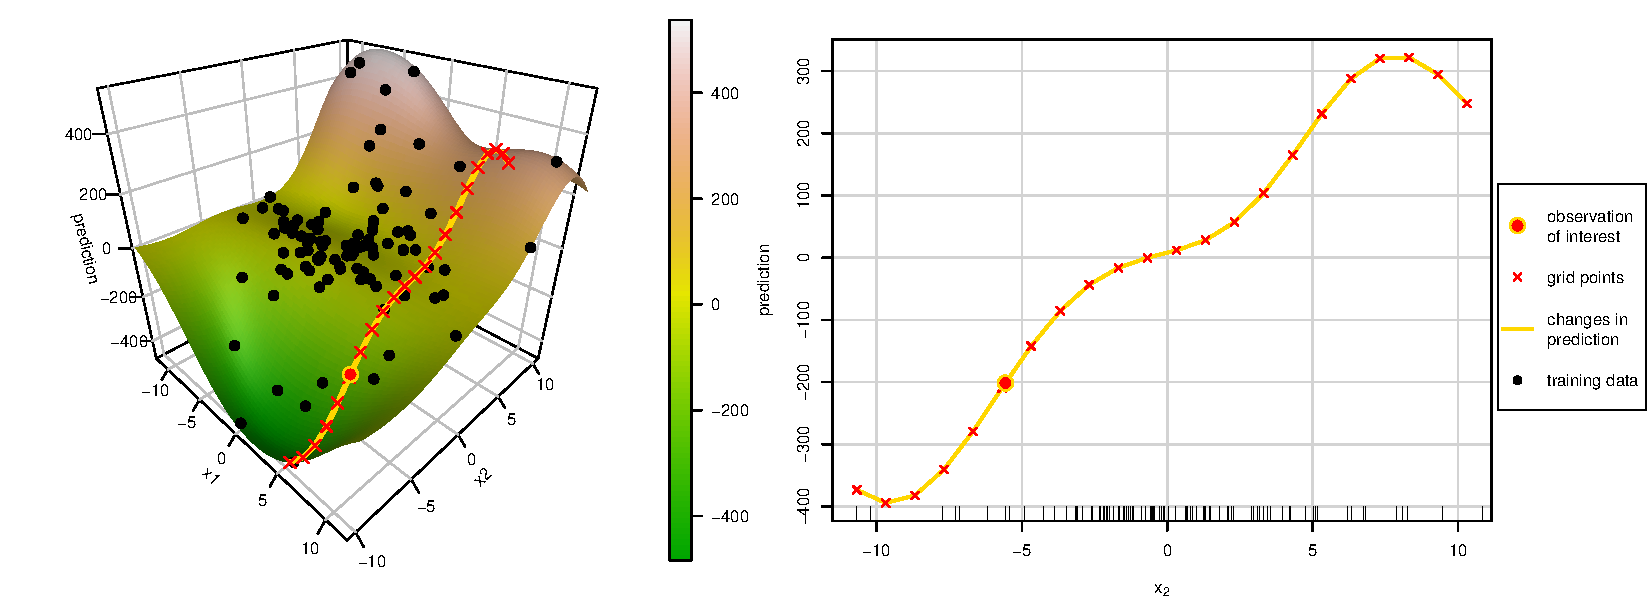
\includegraphics[width=\textwidth]{figure/ice_motivation}

%% Wie nutzt man ICE Kurven zur lokalen Interpretation?
\end{frame}


\begin{frame}{Comments on Grid values}
\begin{itemize}
%\item ICE curves show how different feature values of an observation affect its prediction \newline $\Rightarrow$ \textbf{local interpretation method}
\item Plotting ICE curves involves generating grid values $\xv_S^*$; visualized on x-axis
\item \textbf{Three common strategies} for grid definition:
\begin{itemize}
\item Equidistant grid values within feature range
\item Random samples from observed feature values
\item Quantiles of observed feature values
\end{itemize}
\item \textbf{Marginal realism:} Random and quantile grids better reflect the marginal distribution of $x_S$
        $\Rightarrow$ reduce unrealistic values along $x_S$
%Except equidistant grid, the other two options preserve (approximately) the marginal distribution of feature of interest
%$\Rightarrow$ Avoids unrealistic feature values for distributions with outliers %or dependencies
\item<2> \textbf{However:} For \textbf{correlated features}, extrapolation remains:
%Correlations/interactions $\leadsto$ unrealistic values in all three methods
%(to be addressed with ALE plots later)%Preferable for skewed distributions (with outliers) to avoid using unrealistic feature values.
% \begin{itemize}
% \item equidistant grid values:
% \item sub-sampled grid values:
% \item quantile grid values:
% \end{itemize}
\end{itemize}

\vspace{0.3cm}
\centering
\includegraphics<1>[width=0.85\textwidth, trim=0cm 0cm 0cm 0cm, clip]{figure/sampling2}
\includegraphics<2>[width=0.85\textwidth, trim=0cm 0cm 0cm 0cm, clip]{figure/sampling}


\end{frame}

% bike sharing example + defaults
\begin{frame}{Practical considerations}

\begin{itemize}
  \item \textbf{Grid resolution} (instances $\times$ grid over feature of interest)
        \begin{itemize}
            \item Too coarse $\Rightarrow$ may miss sharp nonlinearities or discontinuities
            %may miss sharp changes%
            \item Too fine $\Rightarrow$ high runtime (without gaining much)
            %time intensive%
            \item Fix: cap at $\approx 50 - 100$ grid points; vectorize predictions by feeding the model a single data frame containing all grid-modified instances
        \end{itemize}
  \item \textbf{ICE curves} (number of instances/curves visualized)
        \begin{itemize}
            \item Too few $\Rightarrow$ hides variability across instances, misses subgroup differences
            %heterogeneity is hidden%
            \item Too many $\Rightarrow$ visual overload (many overlapping curves), time intensive%
            \item Fix: Stratified or cluster-based subsample (e.g., 100); facet by subgroup
        \end{itemize}
\end{itemize}

\begin{columns}[T, onlytextwidth]
\begin{column}{0.5\textwidth}
\small

Default values for popular libraries: 

\medskip

%\centering
\begin{tabular}{lcc}
\textbf{Library} & \textbf{Grid} & \textbf{ICE curves}\\\hline
sklearn (Py) & 100 & 1\,000 (random) \\
PDPbox  (Py) & 10  & num. rows\\
iml (R)      & 20  & num. rows\\
pdp (R)      & 51  & num. rows\\
\end{tabular}

\end{column}

% -------- RIGHT COLUMN: FIGURE --------
\begin{column}{0.5\textwidth}
\centering
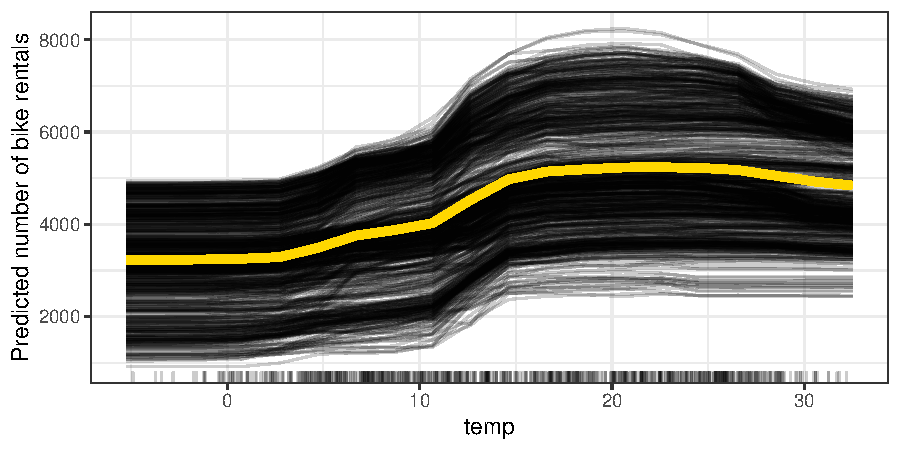
\includegraphics[width=\textwidth]{figure/pdp_bike.pdf}

\end{column}
\end{columns}

\centerline{\small
ICE curves (\textbf{black lines}) and their point-wise average across the grid (\textbf{yellow line})%, known as "partial dependence plot"
}
\end{frame}

\endlecture
\end{document}
